\documentclass[../main.tex]{subfiles}
\begin{document}

\chapter{Рисунок и фон}

\subsection{Простые и составные числа}

ТО, ЧТО некоторые понятия можно выразить при помощи простых манипуляций типографскими символами, кажется довольно странным.
До сих пор мы передали таким образом лишь понятие сложения, и это, возможно, не~показалось нам удивительным.
Предположим, однако, что мы захотим создать формальную систему с теоремами вида \textbf{P$x$}, где~$x$ было бы строчкой, состоящей из тире.
Количество этих тире должно было бы выражаться простым числом.
Так, \textbf{P--{}--} было бы теоремой, в то время как \textbf{P--{}--{}--} теоремой бы не являлось.
Как это может быть выражено с помощью типографских операций?
Сначала необходимо точно определить, что мы имеем в виду под «типографскими операциями».
Полное описание было дано в системах~\textbf{MIU} и~\textbf{pr}, так что сейчас мы ограничимся только списком наших возможностей:

\begin{enumerate}[label=(\arabic*), noitemsep, topsep=6pt]
    \item читать и узнавать любое из конечных множеств символов;
    \item записывать любой из символов, принадлежащий такому множеству;
    \item повторять любой из этих символов в другом месте;
    \item стирать любой из этих символов;
    \item проверять, одинаковы ли два символа;
    \item сохранять и использовать список ранее выведенных теорем.
\end{enumerate}

Список получился немного повторяющимся, но это не столь важно.
Главное то, что он позволяет только самые тривиальные операции, намного проще, чем операция отличения простого числа от не простого.
Как же, в таком случае, мы сможем совместить несколько операций и создать такую формальную систему, в которой простые числа отличались бы от составных?

\subsection{Система~\textbf{ur}}

Первым шагом может стать решение более простой, но сходной задачи.
Мы можем попытаться придумать систему, похожую на систему~\textbf{pr}, но которая вместо сложения представляла бы умножение.
Назовем её системой~\textbf{ur} (u~=~«умноженное на»).
Предположим, что $X$, $Y$, $Z$, соответственно, \--- это количество тире в строчках $x$,~$y$,~$z$.
(Обратите внимание, что я специально делаю упор на различии между строчкой, и количеством тире, которое эта строчка содержит.)
Мы~хотим, чтобы строчка \textbf{$x$u$y$rz} была теоремой только в том случае, когда~$X$, умноженное на~$Y$, равняется~$Z$.
Например, \textbf{--{}--u--{}--{}--r--{}--{}--{}--{}--{}--} должно быть теоремой, так как~2, умноженное на~3, равняется~6, в то время как \textbf{--{}--u--{}--r--{}--{}--} теоремой быть не~должно.
Систему~\textbf{ur} так же просто описать, как и систему~\textbf{pr}.
Для этого нужны всего лишь одна аксиома и одно правило вывода:

\begin{tcolorbox}[title={СХЕМА АКСИОМ}]
    \textbf{$x$u--r$x$} является аксиомой, когда $x$ \--- строчка, состоящая из тире.
\end{tcolorbox}

\begin{tcolorbox}[title={ПРАВИЛО ВЫВОДА}]
    Предположим, что $x$, $y$, и $z$ \--- строчки тире, и что \textbf{$x$u$y$r$z$} \--- старая теорема.
    Тогда \textbf{$x$u$y$--r$zx$} будет новой теоремой.
\end{tcolorbox}

Ниже приводится вывод теоремы \textbf{--{}--u--{}--{}--r--{}--{}--{}--{}--{}--}:
\begin{center}
\begin{tabular}{r @{~} l @{~~} l}
    (1) & \textbf{--{}--u--r--{}--}
        & (аксиома) \\
    (2) & \textbf{--{}--u--{}--r--{}--{}--{}--}
        & (по правилу вывода, используя (1) в качестве старой теоремы) \\
    (3) & \textbf{--{}--u--{}--{}--r--{}--{}--{}--{}--{}--}
        & (по правилу вывода, используя (2) в качестве старой теоремы) \\
\end{tabular}
\end{center}
Обратите внимание, что количество тире в средней строке возрастает на единицу каждый раз, когда мы применяем правило вывода, таким образом, мы можем предсказать, что если мы хотим получить теорему с десятью тире в середине, нам придется применить правило вывода девять раз подряд.


\subsection{Уловление Составности}

Умножение (немного более сложное понятие, чем сложение) теперь уловлено нами в сети типографских правил, подобно птицам в Эшеровском «Освобождении».
А как же насчет простых чисел?
Следующий план кажется неплохим: используя систему \textbf{ur} , определить новое множество теорем вида S$x$, которые характеризуют \emph{составные числа}.

\begin{tcolorbox}[title={ПРАВИЛО}]
    Предположим, что $x$, $y$, $z$ \--- строчки тире.
    Если \textbf{$x$--u$y$--r$z$} является теоремой, то S$z$ также будет теоремой.
\end{tcolorbox}

Это означает, что $Z$ (число тире в~$z$) является составным, если оно \--- произведение двух чисел, больших единицы (а именно, $X + 1$ \--- число тире в~\textbf{--$x$} и $Y + 1$ \--- число тире в~\textbf{$y$--}).
Я~объясняю вам это новое правило в «интеллектуальном режиме», поскольку вы, как существо мыслящее, желаете знать, почему такое правило существует.
Если бы вы работали исключительно в «механическом режиме», вам бы не понадобились никакие объяснения, так как работающие в режиме~\textbf{M} следуют правилам чисто механически, никогда не задавая вопросов, и при этом совершенно счастливы!

Поскольку вы работаете в режиме \textbf{I}, вы будете склонны забывать о различии между строчками и их интерпретацией. Ситуация может стать довольно запутанной, как только вы обнаружите смысл в символах, которыми вы манипулируете.
Вам придется бороться с собой, чтобы не решить, что строчка «\textbf{--{}--{}--»}--- то же самое, что число~3.
% TODO: add ref?
Требование формальности, казавшееся совершенно очевидным в главе I, здесь становится весьма каверзным и приобретает первостепенную важность.
Именно оно не дает вам спутать режим~\textbf{I} с режимом~\textbf{M}, иными словами, оно не позволяет вам смешивать арифметические факты с типографскими теоремами.


\subsection{«Нелегальная» характеристика простых чисел}

Весьма соблазнительно от теорем типа~S сразу перескочить к теоремам типа~P, путем введения следующего правила

\begin{tcolorbox}[title={ПРЕДЛОЖЕННОЕ ПРАВИЛО}]
    Предположим, что $x$ \--- строчка тире.
    Если S$x$ не является теоремой, то P$x$ является теоремой.
\end{tcolorbox}

Роковая ошибка здесь заключается в том, что проверка «нетеоремности» S$x$ \--- не~типографская операция.
Чтобы узнать наверняка, что \textbf{MU} \--- не теорема \textbf{MIU}, нам пришлось бы \emph{выйти из системы}; в такую же ситуацию мы попадаем и с Предложенным Правилом.
Оно подрывает сами основы формальных систем тем, что предлагает вам действовать неформально, вне системы.
Типографская операция (6) позволяет вам рассматривать предварительно выведенные теоремы; однако Предложенное Правило отсылает вас к гипотетической «таблице не-теорем».
Чтобы получить подобную таблицу, вам придется работать \emph{вне~системы}, показывая, почему некоторые строчки не~могут быть получены в данной системе.
Конечно, может оказаться, что существует другая формальная система, в которой «таблица не-теорем» может быть получена чисто~типографскими способами.
На самом деле, наша цель \--- найти именно такую систему.
Однако Предложенное Правило \--- не~типографское, а посему нам придется от него отказаться.

Это настолько важный момент, что мы остановимся на нем поподробнее.
В нашей \emph{системе~S} (включающей систему~\textbf{ur} и правила, определяющие теоремы типа S) у нас есть теоремы вида~S$x$, где~$x$, как обычно, обозначает строчку тире.
В ней имеются также не-теоремы вида S$x$.
Говоря о не-теоремах, я имею в виду именно эту разновидность, хотя, конечно, существует множество не-теорем в виде неправильно сформированных строчек: \textbf{uu--Srr} и~пр.
Между теоремами и не-теоремами есть следующая разница: количество тире в первых \--- составное число, во вторых \--- простое.
К тому же, все теоремы похожи по форме, так как все они выведены при помощи одного и того же набора типографских правил.
Можем ли мы сказать, что в этом смысле все не-теоремы также имеют что-то общее в форме?
Ниже приводится список теорем типа~S, без их вывода.
Число в скобках указывает на количество тире в соответствующей теореме.

\begin{center}
\begin{minipage}{0.4\textwidth}
    S\textbf{--{}--{}--{}--} (4)

    S\textbf{--{}--{}--{}--{}--{}--} (6)

    S\textbf{--{}--{}--{}--{}--{}--{}--{}--} (8)

    S\textbf{--{}--{}--{}--{}--{}--{}--{}--{}--} (9)

    S\textbf{--{}--{}--{}--{}--{}--{}--{}--{}--{}--} (10)

    S\textbf{--{}--{}--{}--{}--{}--{}--{}--{}--{}--{}--{}--} (12)

    S\textbf{--{}--{}--{}--{}--{}--{}--{}--{}--{}--{}--{}--{}--{}--} (14)

    S\textbf{--{}--{}--{}--{}--{}--{}--{}--{}--{}--{}--{}--{}--{}--{}--} (15)

    S\textbf{--{}--{}--{}--{}--{}--{}--{}--{}--{}--{}--{}--{}--{}--{}--{}--} (16)

    S\textbf{--{}--{}--{}--{}--{}--{}--{}--{}--{}--{}--{}--{}--{}--{}--{}--{}--{}--} (18)
\end{minipage}

$\vdots$
\end{center}

«Дырки» в этом списке как раз и являются не-теоремами. Есть ли у них какая-то общая «форма»? Можно ли предположить, что лишь постольку, поскольку они являются пробелами в неком упорядоченном списке, они обладают какими-то общими чертами? И да, и нет. Нельзя отрицать, что у них есть общие типографские черты; вопрос в том, правомочно ли называть эти черты «формой». Дело в том, что дырки определены только негативно: они представляют из себя то, что осталось от позитивно определенного списка.


\subsection{Рисунок и фон}

Это напоминает известное разграничение между рисунком и фоном в живописи.
Когда предмет или «положительное пространство» (например, человеческая фигура, буква или натюрморт) рисуется внутри рамки, неизбежным следствием этого является появление на картине дополняющей формы, также называющейся «фоном», или «негативным пространством».
В большинстве картин отношение между фоном и рисунком почти не играет роли; как правило, художник в основном занят рисунком.
Однако иногда его внимание привлекает также и фон.

Существуют замечательные шрифты, обыгрывающие это различие между рисунком и фоном.
Послание, написанное таким шрифтом, приводится ниже.
На первый взгляд это просто несколько клякс; но если вы посмотрите на них издали, попристальнее, то увидите семь букв на этом РИСУНКЕ (специальным шрифтом, так, что черный фон, создающий белые буквы, похож на кляксы.)

\emph{Рис. 15. Рисунок}

Такой же эффект производит мой рисунок «Знак из дыма» (рис. 139).
Продолжая в том же ключе, попробуйте решить следующую задачку: возможно ли нарисовать такую картину, чтобы слова были как на рисунке, так и в фоне?

Давайте условимся различать между двумя типами рисунков: \emph{курсивно рисуемыми} и \emph{рекурсивными} (эти термины не~являются общеупотребительными \--- их придумал я сам).
В~\emph{курсивно рисуемом} рисунке фон является лишь побочным продуктом.
В~\emph{рекурсивном} рисунке, наоборот, фон может рассматриваться как отдельный самостоятельный рисунок. Обычно художник делает это вполне сознательно.
Приставка «ре» здесь выражает тот факт, что как рисунок, так и фон могут быть нарисованы курсивно, то~есть, такая картина «дву-курсивна».
Любой контур на рекурсивном рисунке \--- это обоюдоострый меч.
М.К.~Эшер был мастером подобных картин; взгляните, например, на его великолепную рекурсивную гравюру «Птицы» (рис.~\ref{fig:escher-birds}).

\begin{figure}
    \centering
    \includegraphics[max width=\linewidth, max totalheight=\textheight-2\baselineskip]{img/escher-birds.png}
    \caption{M.K. Эшер. «Деление пространства при помощи птиц» (из блокнота 1942 года)}
    \label{fig:escher-birds}
\end{figure}

Различие здесь не такое строгое, как в математике; кто может с уверенностью утверждать, что некий фон не является в то же время и рисунком?
При достаточно внимательном рассмотрении, любой фон не лишен собственного интереса.
В~этом смысле любой рисунок можно назвать рекурсивным.
Однако, вводя эти термины, я~имел в виду нечто другое.
Существует естественное, интуитивное понятие узнаваемых форм.
Являются ли и рисунок и фон узнаваемыми формами?
Если да, то такой рисунок рекурсивен.
Посмотрев на фон большинства контурных рисунков, вы обнаружите, что в нем трудно признать какую-либо форму.
Это доказывает, что:
%
\begin{block}
    Существуют узнаваемые формы, чье негативное пространство не является никакой узнаваемой формой.
\end{block}
%
Или, выражаясь более технично:
%
\begin{block}
    Существуют курсивно рисуемые рисунки, которые не рекурсивны.
\end{block}

\emph{Рис. 17. Скотт Е. Ким Рисунок «РИСУНОК-РИСУНОК».}

На рис. 17 показано решение предложенной выше головоломки, принадлежащее Скотту Киму; я называю это решение «рисунок РИСУНОК--РИСУНОК».
На какую бы часть \--- белую или черную \--- вы не посмотрели, вы увидите только «ФИГУРЕ» (=~английское «РИСУНОК»), и никакого «ФОНА».
Великолепный образчик рекурсивного рисунка!
Черные области этого хитроумного рисунка можно охарактеризовать двумя способами:
%
\begin{enumerate}[label=(\arabic*), noitemsep, topsep=6pt, left=\parindent]
    \item как \emph{негативное пространство} белых областей;
    \item как \emph{видоизмененные копии} белых областей (полученные путем их окраски и сдвига каждой белой области).
\end{enumerate}
%
(В данном случае обе характеристики эквивалентны; для большинства черно-белых рисунков это не так.)
% TODO: add ref?
В главе VIII, создавая Типографскую Теорию Чисел (ТТЧ), мы будем надеяться, что нам удастся охарактеризовать множество всех ложных утверждений аналогичными способами:
%
\begin{enumerate}[label=(\arabic*), noitemsep, topsep=6pt, left=\parindent]
    \item как \emph{негативное пространство} множества всех теорем ТТЧ;
    \item как \emph{модифицированные копии} множества всех теорем ТТЧ (полученные путем отрицания каждой теоремы ТТЧ).
\end{enumerate}
%
Однако этой надежда окажется напрасной, так как:
%
\begin{enumerate}[label=(\arabic*), noitemsep, topsep=6pt, left=\parindent]
    \item среди множества всех не-теорем существуют некоторые истинные утверждения;
    \item вне множества всех отрицаний теорем, существуют некоторые ложные утверждения.
\end{enumerate}

% TODO: add ref?
Отчего так получается, вы увидите в главе XIV; а пока можете поразмыслить над графическим изображением данной ситуации (Рис.~\ref{fig:formulae}).

\begin{figure}
    \centering
    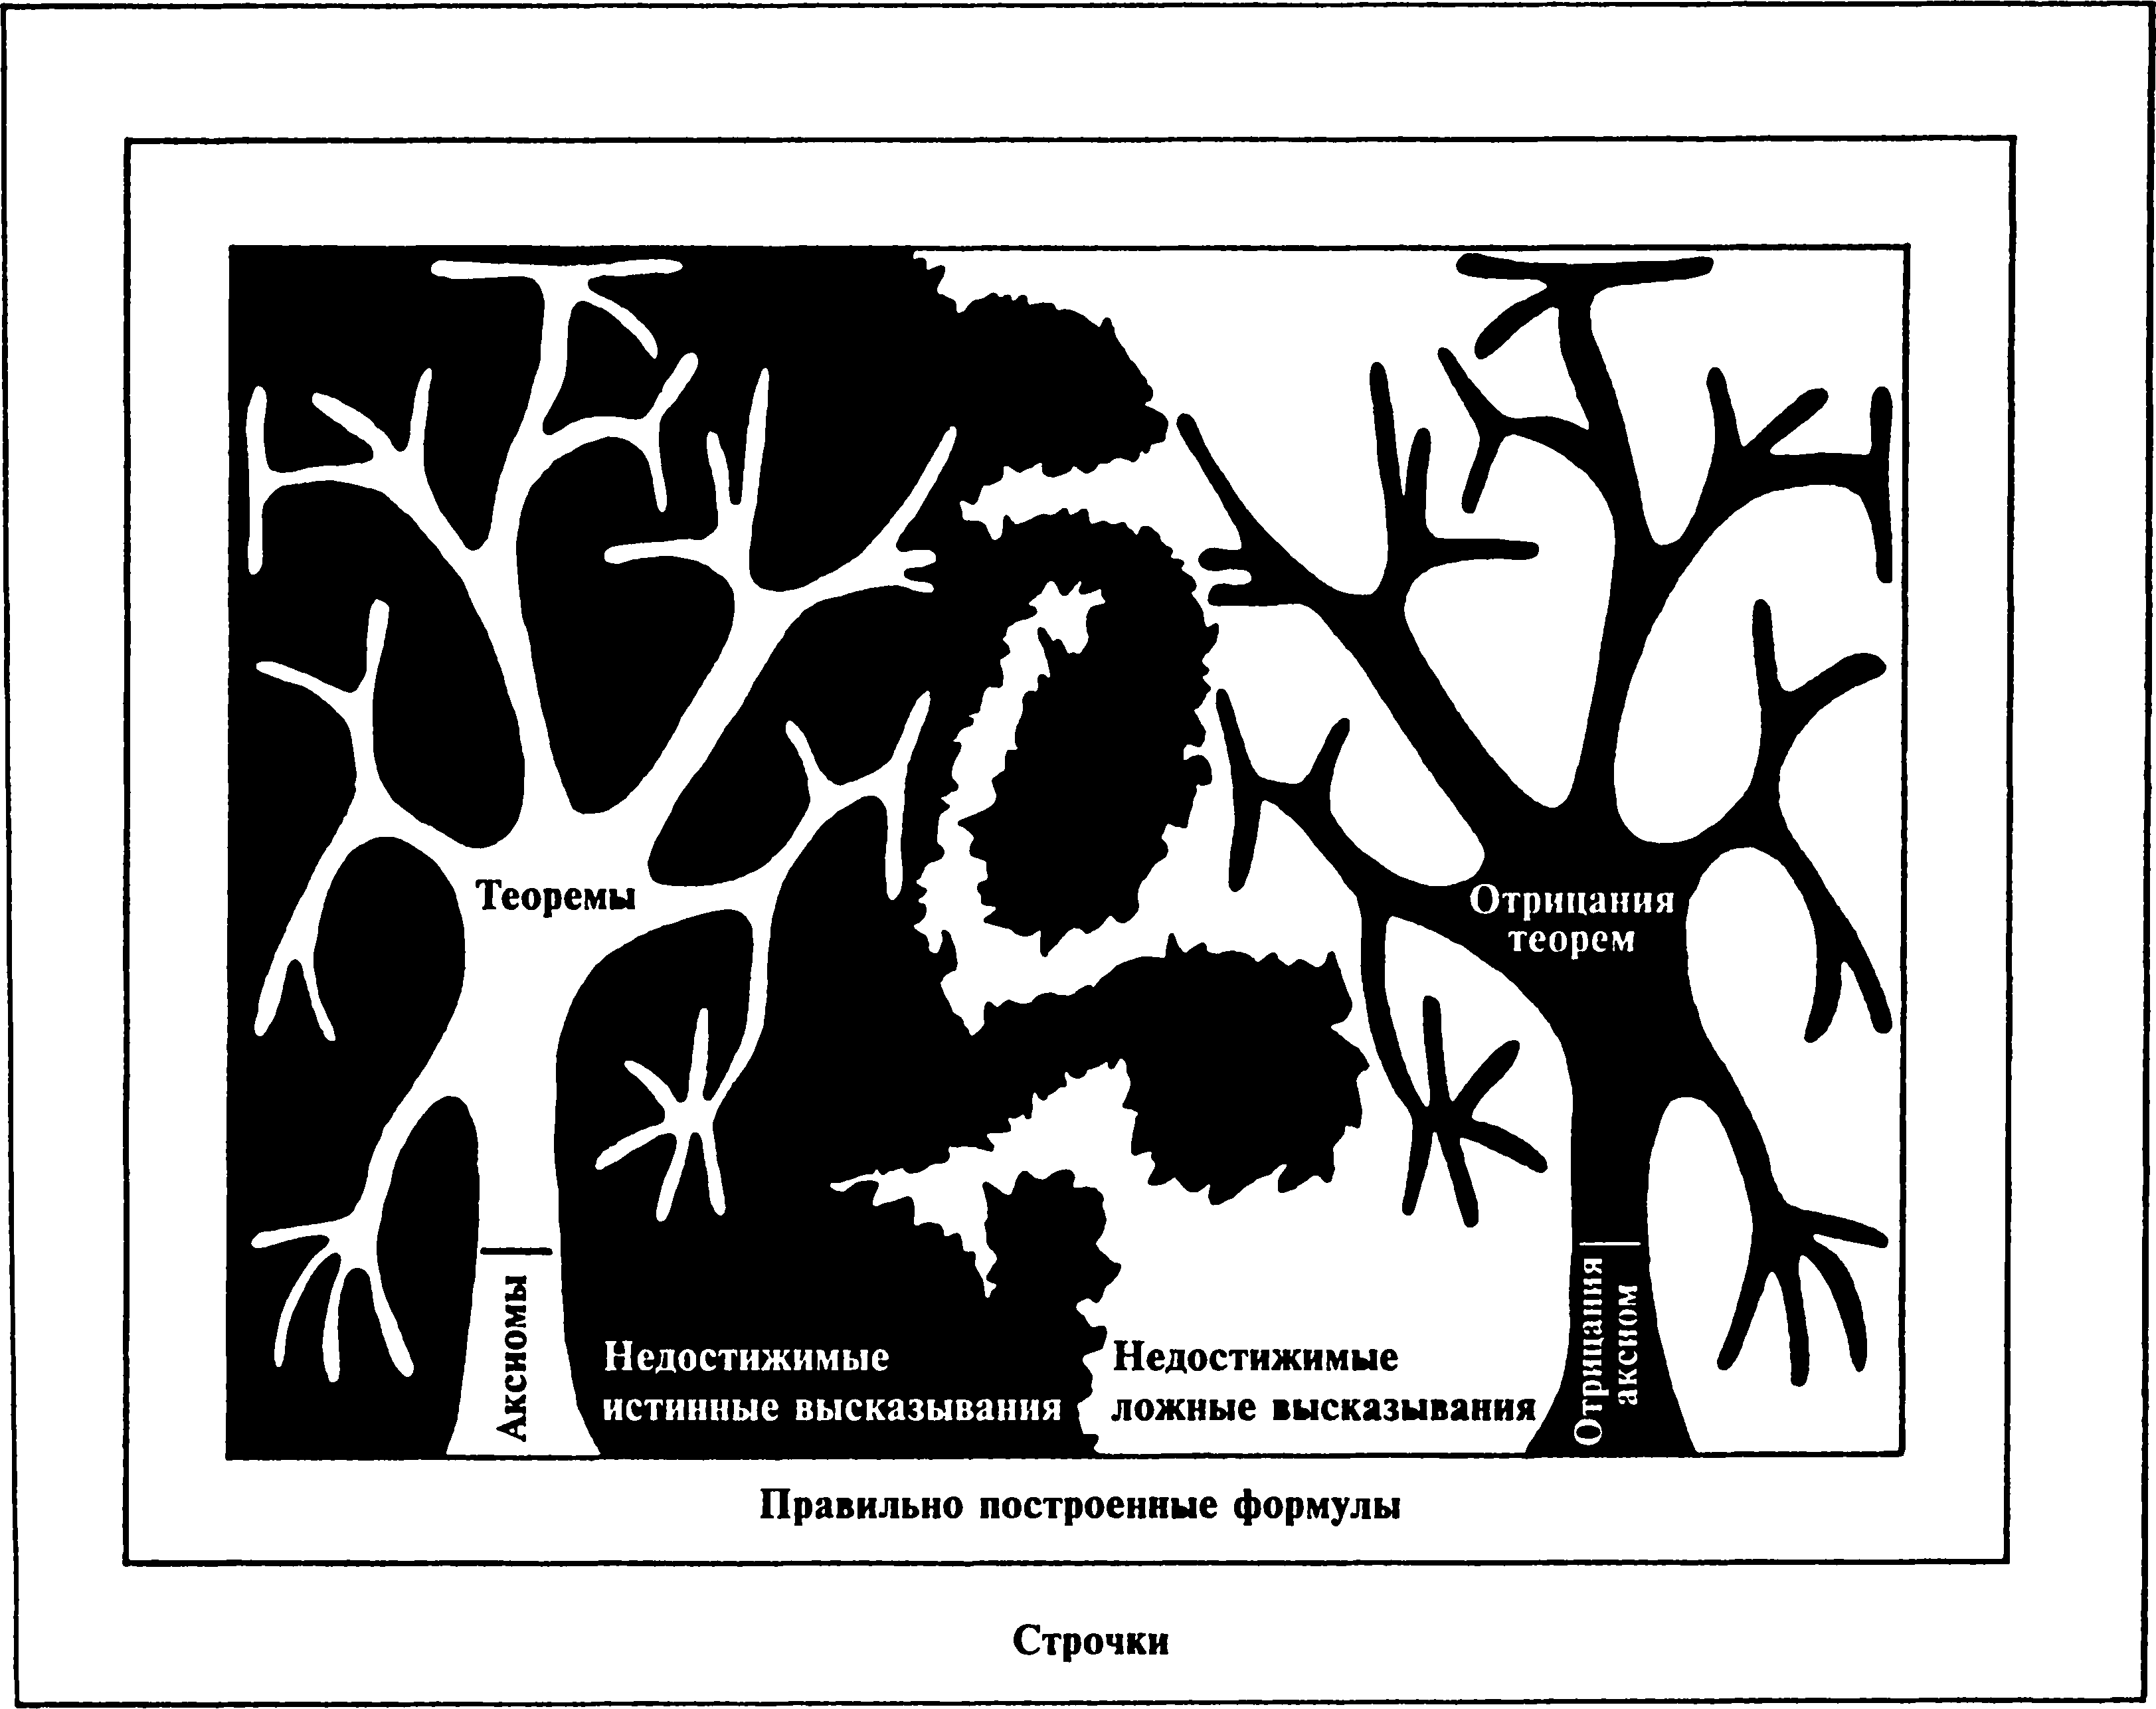
\includegraphics[width=\textwidth, max totalheight=\textheight-2\baselineskip]{img/formulae.png}
    \caption{Эта диаграмма отношений между различными классами строчек ТТЧ весьма богата зрительным символизмом. Самый большой прямоугольник \--- множество всех строчек ТТЧ\@. Следующий прямоугольник \--- все правильно построенные строчки ТТЧ\@. Внутри него находится множество всех предложений ТТЧ\@. Именно на этом уровне начинают происходить интересные вещи. Множество теорем изображено в виде дерева, чей ствол \--- множество аксиом. Символ дерева был выбран из-за того, что оно растет «рекурсивно» новые ветви (теоремы) вырастают из старых. Пальцеобразные ветви проникают во все уголки области представляющей множество истинных высказываний, однако они не могут занять эту область целиком. Граница между областями истинных и ложных высказываний представляет собой изломанную «береговую линию», которая, как бы близко вы её не рассматривали, всегда имеет ещё более мелкие уровни структуры и таким образом, не поддается описанию каким либо конечным методом (См.~книгу Мандельбродта «Фракталы» (В.~Mandelbrodt Fractals)). Отраженное дерево справа представляет отрицания теорем все они ложны, но вкупе они не в состоянии заполнить всю область ложных высказываний (Рисунок~автора)}
    \label{fig:formulae}
\end{figure}


\subsection{Рисунок и фон в музыке}

Аналогию с понятием рисунка и фона можно также найти и в музыке.
Примером может служить различие между мелодией и аккомпанементом: мелодия всегда на первом плане, тогда как аккомпанемент в каком-то смысле второстепенен.
Поэтому нам кажется удивительным, когда мы узнаем мелодии на «низшем» уровне музыкального произведения.
Для пост-барочной музыки это редкое явление \--- обычно гармонии там не выходят на первый план.
Но в барочной музыке \--- и прежде всего, у Баха \--- все уровни «работают» в качестве «рисунка».
В этом смысле баховские композиции могут быть названы рекурсивными.

В музыке есть ещё одно различие между рисунком и фоном \--- ударные и безударные такты.
Если вы начнете отмечать ритм счетом «раз-и, два-и, три-и\ldots», большинство нот мелодии придутся на числа, а не на «и».
Иногда, однако, мелодия бывает нарочно смещена на «и», чем достигается интересный эффект.
Это происходит, например, в нескольких фортепианных этюдах Шопена.
Тот же прием можно найти у Баха, в особенности, в сонатах и партитурах для скрипки соло и в сюитах для виолончели соло.
В этих композициях Баху удается поместить несколько мелодий одновременно на разных уровнях.
Иногда он достигает этого эффекта, заставляя солирующий инструмент играть дублировки \--- две ноты сразу.
В других случаях, однако, он помещает один голос на ударные такты, а другой \--- на безударные, так что слух различает две разные мелодии, вплетающиеся одну в другую и гармонически сочетающиеся.
Нет нужды говорить, что Бах не останавливается на этом уровне сложности\ldots{}


\subsection{Рекурсивно счетные и рекурсивные множества}

Перенесем понятие рисунка и фона обратно в область формальных систем.
В нашем примере роль позитивного пространства играют теоремы типа~S, а роль негативного пространства \--- строчки, в которых количество тире выражается простым числом.
Пока что единственный способ, который нам удалось найти для выражения простых чисел типографским путем, это негативное пространство.
Существует ли какой нибудь способ выразить простые числа в виде позитивного пространства, то есть в виде множества теорем некой системы?

Интуиция подсказывает разным людям разные ответы.
Я отчетливо помню, как был озадачен и заинтригован, заметив разницу между негативной и позитивной характеристиками.
Я был совершенно уверен в том, что не только простые числа, но и вообще любое негативно определяемое множество чисел может быть определено позитивно.
Интуитивное обоснование моей уверенности заключалось в следующем вопросе: «\emph{Как это возможно, чтобы рисунок и фон не содержали совершенно одинаковой информации}?»
Мне казалось, что они представляют собой одну и ту же информацию, закодированную двумя разными способами.
А что думаете по этому поводу вы, читатель?

Выяснилось, что я был прав насчет простых чисел, но ошибался в остальном. Тогда это меня поразило и продолжает поражать и по сей день.
Оказывается, что:
%
\begin{block}
    существуют такие формальные системы, чье негативное пространство (множество не-теорем) не является позитивным пространством никакой другой формальной системы.
\end{block}

Как выяснилось, этот результат сравним по глубине с Теоремой Гёделя \--- так что неудивительно, что моя интуиция не могла принять его сразу.
Подобно математикам начала двадцатого века, я считал мир формальных систем и натуральных чисел более предсказуемым, чем он оказался в действительности.
Выраженное более техническим языком, это утверждение звучит так:
%
\begin{block}
    Существуют рекурсивно счетные множества, не являющиеся рекурсивными.
\end{block}

Выражение «рекурсивно счетные» (часто сокращаемое как р.с.) \--- математическое соответствие нашему художественному понятию «курсивно рисуемые», а \emph{рекурсивный} \--- соответствие «рекурсивным».
Множество строчек является р.с., когда все они могут быть выведены путем применения типографских правил \--- например, множество теорем типа S или множество теорем системы~\textbf{MIU}; на самом деле, это определение приложимо ко множеству теорем любой формальной системы.
Оно сравнимо с понятием о «рисунке» как о «множестве линий, которые могут быть произведены в соответствии с художественными правилами» (что бы это последнее не означало!).
А~«рекурсивное множество» подобно рисунку, чей фон, в свою очередь, также является рисунком \--- в таком случае не только рисунок, но и его дополнение будут р.с.

Из этого вытекает следующий результат:
%
\begin{block}
    Существуют такие формальные системы, у которых нет типографского алгоритма разрешения.
\end{block}
%
Из чего это следует?
Очень просто.
Типографский алгоритм разрешения \--- это метод, отличающий теоремы от не-теорем.
Он позволяет нам выводить не-теоремы систематически, идя по списку \emph{всех} строчек и отбрасывая те, что не являются теоремами.
Эту процедуру можно назвать типографским методом вывода множества не-теорем.
Однако из предыдущего утверждения (которое мы пока принимаем на веру) следует, что для \emph{некоторых} формальных систем это невозможно.

Предположим, что мы нашли множество~$R$ («$R$» \--- рисунок) натуральных чисел, которое мы можем вывести каким-либо формальным путем \--- вроде множества составных чисел. Предположим, что его дополнением является множество~$F$ («$F$» \--- фон) \--- простые числа.
Вместе взятые, $R$~и~$F$ дают все натуральные числа.
Мы знаем правило, позволяющее вывести все числа множества~$R$, для чисел множества~$F$ такого правила не существует.
Важно, что если числа~$R$ выводятся исключительно \emph{в возрастающем порядке}, то мы всегда можем охарактеризовать~$F$.
Трудность заключается в том, что многие р.с. множества производятся при помощи таких методов, которые выводят элементы в произвольном порядке, так что не известно, появится ли какое-либо число, до сих пор пропускаемое, если подождать ещё чуть-чуть.

На вопрос «Все ли рисунки рекурсивны?» мы ответили отрицательно.
Теперь мы видим что придется ответить отрицательно и на аналогичный вопрос математиков «Все ли множества рекурсивны?»
Имея это в виду, давайте вернемся к этому расплывчатому понятию «формы».
Обратимся снова к нашим множествам: $R$ \--- рисунки и $F$ \--- фон.
Легко согласиться с тем, что все числа во множестве~$R$ имеют какую-то общую «форму» \--- но можно ли сказать то же самое о числах множества~$F$?
Странный вопрос.
С самого начала имея дело с бесконечным множеством всех натуральных чисел, весьма сложно прямо и четко определить «дырки», остающиеся в списке после изъятия оттуда неких чисел.
Таким образом, возможно что на самом деле у этих дырок нет никаких общих характеристик «формы».
Неясно, стоит ли вообще использовать здесь такое соблазнительное словечко как «форма».
Может быть лучше не определять этого понятия оставив ему некую интуитивную гибкость.

Вот вам ещё одна головоломка, над которой вы можете поразмыслить в связи с изложенным выше.
Можете ли вы охарактеризовать следующее множество чисел (или его негативное пространство)?
\[
    1 \quad 3 \quad 7 \quad 12 \quad 18 \quad 26 \quad 35 \quad 45 \quad 56 \quad 69
\]
Чем данная последовательность напоминает рисунок РИСУНОК--РИСУНОК?


\subsection{Простые числа в качестве рисунка, а не фона}

Как же насчет формальной системы для вывода простых чисел?
Как это сделать?
Способ состоит в том чтобы, не останавливаясь на умножении, обратиться прямо к неделимости, представив её позитивно.
Ниже дана схема аксиом и правило вывода теорем, представляющих понятие числа, не являющегося делителем других чисел (\textbf{ND}~=~не~делитель).

\begin{tcolorbox}[title={СХЕМА АКСИОМ}]
    \textbf{$xy$ND$x$}, где $x$ и $y$ \--- строчки тире.
\end{tcolorbox}

Например, \textbf{--{}--{}--{}--{}--ND--{}--} , где $x$ заменен на «\textbf{--{}--»} и $y$ \--- на «\textbf{--{}--{}--»}

\begin{tcolorbox}[title={ПРАВИЛО}]
    Если \textbf{$x$ND$y$} является теорема, то \textbf{$x$ND$xy$} также будет теоремой.
\end{tcolorbox}

Приложив это правило дважды, вы можете вывести теорему
%
\begin{center}
    \textbf{--{}--{}--{}--{}--ND--{}--{}--{}--{}--{}--{}--{}--{}--{}--{}--{}--}
\end{center}
%
которая интерпретируется как «5~не~делитель~12».
Однако \textbf{--{}--{}--ND--{}--{}--{}--{}--{}--} не~является теоремой.
В чем будет ошибка, если вы попытаетесь вывести эту строчку?

Чтобы определить, что данное число простое, у нас должны быть какие-то сведения о его свойствах неделимости.
В частности, мы хотим знать, что это число не делится на 2, 3, 4, и т.~д., до числа, меньшего его на единицу.
Однако в формальных системах мы не можем позволить себе таких расплывчатых формулировок как «и~так далее».
Здесь нужна исчерпывающая точность.
Нам бы хотелось иметь возможность сказать на языке системы: «число~$Z$ \emph{свободно от делителей} до~$X$» (\textbf{SOD}~=~свободно от делителей), имея в виду, что не одно число между 2 и~$X$ не является делителем $Z$.
Это можно сделать, но здесь есть небольшой трюк.
Если хотите, можете попытаться найти его.

Решение заключается в следующем:

\begin{tcolorbox}[title={ПРАВИЛО 1}]
    Если \textbf{--{}--ND$z$} является теоремой, то \textbf{$z$SOD--{}--} также будет теоремой.
\end{tcolorbox}

\begin{tcolorbox}[title={ПРАВИЛО 2}]
    Если \textbf{$z$SOD$x$} и \textbf{$x$--ND$z$} являются теоремами, то \textbf{$z$SOD$x$} также будет теоремой.
\end{tcolorbox}

Эти два правила, в совокупности, характеризуют понятие свободы от делителей.
Все что нам нужно, это указать, что простые числа \--- это числа, \emph{свободные от делителей}, включая число на единицу меньшее их самих:

\begin{tcolorbox}[title={ПРАВИЛО 3}]
    Если \textbf{$z$--SOD$z$} является теоремой, то \textbf{P$z$--} также будет теоремой.
\end{tcolorbox}

Не будем забывать, что 2 \--- тоже простое число!

\begin{tcolorbox}[title={АКСИОМА}]
    \textbf{P--{}--}
\end{tcolorbox}

Вот и все, что нам необходимо.
Принцип формального выражения «просто-численности» заключается в том, что существует метод проверки, не~требующий никакого отступления назад.
Вы всегда двигаетесь вперед, проверяя данное число на делимость \--- сначала на~2, потом на~3, и так далее.
Именно эта «монотонность» или однонаправленность \--- отсутствие игры между укорачивающими и удлиняющими правилами \--- позволила нам уловить суть простых чисел.
И именно этой потенциальной сложностью формальных систем, могущих вместить сколько угодно взаимодействий между движением вперед и назад, объясняются такие ограничивающие результаты как Теорема Гёделя и Проблема Остановки Тюринга, как и тот факт, что не все рекурсивно счетные множества рекурсивны.

\end{document}
